\documentclass[12pt,a4paper]{article}

% incluyendo paquetes
\usepackage[utf8]{inputenc}
\usepackage[spanish]{babel}
\usepackage{milibreria}
 

\graphicspath{{C:/Users/HUAWEI/Pictures/imagesppt/}} %\incluye todos las imágenes de esa ruta
%\graphicspath{{D:/proyectos_latex/7mo_semestre/gestion_redes/informe_de_redes/main/images}}
\begin{document} % inicio  de documento 



\begin{titlepage}
    %\begin{tikzpicture}[overlay, remember picture]
    %    \fill[red] (10cm,-10cm) rectangle (5cm,-15cm);
    %\end{tikzpicture}
    
    \miRectangulo{-2cm}{-4cm}{2cm}{5cm}{rosado}
%   \miRectangulo{x     }{y }{x1    }{y1   }{color}
    
    \miRectangulo{-1.5cm}{-2cm}{-1.2cm}{23.5cm}{black} % 1
    \miRectangulo{-1.8cm}{23.5cm}{5.7cm}{23.2cm}{black} % 2
    \miRectangulo{5.025cm}{23.5cm}{5.33cm}{20cm}{black} % 3
    \miRectangulo{-2.7cm}{-1.7cm}{4.7cm}{-2cm}{black} % 4
    \miRectangulo{4.2cm}{-2cm}{4.5cm}{10cm}{black} % 5

    \begin{textblock}{100}(100,20)
        \begin{flushright}
        {\huge{\textbf{Universidad Nacional del Altiplano}}}\\
        {\normalsize{\textbf{Educando mentes, Cambiando el mundo}}}
        \end{flushright}
        
    \end{textblock}
    
    \begin{tikzpicture}[remember picture, overlay]
        \node at (current page.north west) [anchor=north west, xshift=120mm, yshift=-47mm] {\includegraphics[width=0.45\textwidth]{\logoright}};
    \end{tikzpicture}
    \begin{textblock}{100}(100,130)
        \begin{flushright}
            {\Large{\textbf{Facultad de Ingeniería Mecánica Eléctrica,
                    Electrónica y Sistemas}}}\\[10pt]
            {\large{\textbf{Escuela Profesional de Ingeniería\\ de Sistemas}}}
        \end{flushright}
    \end{textblock}

    \begin{textblock}{200}(10,163)
        \begin{center}
            
            %\textcolor{azul}{\rule{\linewidth}{0.80mm}}
            % titulo del articulo
            %Monitoreo de la atención de los estudiantes mediante cámaras y celulares dentro del Aula en Puno Perú  \par
            \vspace*{\fill}
                \begin{minipage}{0.9\textwidth}
                    \centering
                    {\Large {\textbf{Auditoria de sistemas para la organizacion de la direccion de proyeccion social y extensio cultural en el ambito de seguridad}}}\par
                \end{minipage}
            \vspace*{\fill}
            \textcolor{azul}{\rule{0.5\linewidth}{0.80mm}} \par
            \vspace{8mm}
            {\large{\textbf{ AUDITORÍA DE SISTEMAS }}} \\[10pt]
            {\large{\textbf{\textcolor{azul}{Ing. TICONA YANQUI FIDEL ERNESTO }}}} \\[20pt]
            {\large{\textbf{estudiante}}}\\[10pt]
            {\large{\textbf{$\looparrowright$   Larota Pilco David Brahyan  $\looparrowleft$ }}}\\[5pt]
            %{\large{\textbf{$\looparrowright$    Quispe Calcina Royer $\looparrowleft$ }}}\\[5pt]
            %{\large{\textbf{$\looparrowright$    Rojas Alejo Bruno $\looparrowleft$ }}}\\[5pt]
            %{\large{\textbf{$\looparrowright$  $\mathfrak{David\ Brahyan\ Larota\ Pilco}$   $\looparrowleft$ }}}\\[20pt]
            \today

        \end{center}
    \end{textblock}
\end{titlepage}
%//--------------------------------------
%@article{prueba,
%  title={prueba del documento lenguaje Latex},
%  author={Autor},
%  journal={https://www.overleaf.com/},
%  volume={13},
%  number={36},
%  pages={34--36},
%  year={2022}
%\lstset{language=SQL}
%\begin{lstlisting}
%\end{lstlisting}
%\lstset{language=Python}
%\lstinputlisting{hilosBancaria.py}
%}
%
%
%\begin{figure}[h]
%    \centering
%    \includegraphics[width=0.5\textwidth]{images/medicion_con_tacometro.png}
%    \caption{se realizo la medición con el tacómetro} 
%\end{figure}
%
%\begin{tabular}{ l c l }
%Tipo  			& = & 	GL-90L-4B5 \\
%Ip              & = &	55 \\
%Cos  $\varphi$    & = &  	  0.78 \\
%Voltaje         & = &	 230/400V \\
%Potencia	    & = &	2HP \\
%Intensidad    	& = & 	6.1/3.5 \\
%Frecuencia  	& = & 	60HZ \\
%Rpm     		& = &	1680 
%\end{tabular} % incluyendo la caratula
\tableofcontents % índice automático
\pagestyle{fancy} \mystyle \newpage % Aplicar el estilo de encabezado y pie de página
% inicio del documento  
\newcounter{step}
\newcommand{\dpsec}{Dirección de Proyección Social y Extensión Cultural}


\section{I. Planificación de la Auditoria}

\section{Información de la organización}
\subsection{Modelamiento De La Empresa}
\subsubsection{Nombre De La Organización}
\textbf{\dpsec}

\subsubsection{Descripción de la Empresa}
La Dirección de Proyección Social y Extensión Cultural, es un órgano dependiente del Vicerrectorado Académico \cite{mysql}, responsable de promover, organizar, dirigir y supervisar las actividades en el marco del desarrollo sostenible de Proyección Social y Extensión Cultural de la universidad, orientados hacia la comunidad, con el fin de coadyuvar al desarrollo de la región, revalorando la identidad cultural.

\subsubsection{Misión, Visión y Valores}
\subsection*{Misión}
La Dirección de Proyección Social y Extensión Cultural es generadora de la interacción con la comunidad para el desarrollo regional a través de la ciencia, la tecnología y las expresiones culturales como parte de la labor académica y de investigación en el marco de la proyección social y extensión cultural sostenible.

\subsubsection*{Visión}
La Dirección de Proyección Social y Extensión Cultural fortalece el desarrollo de la región, bajo los principios de la ciencia, la tecnología, los valores culturales y la investigación en el marco de una responsabilidad social sostenible.

\subsection{Servicios y registro institucional}
%\subsubsection{Información Escale (Organización)}
\subsubsection{Horarios de Atencion, Contactos, Portar WEB}
\begin{table}[!hbt]
    \centering
    \begin{tabular}{cc}
    \toprule
    \textbf{Nombre } & \textbf{Información} \\ 
    \midrule
    Dirección: & Auditorio Magno UNAP, Puno 21001 \\
    Directora & DRA. MILDER ZANABRIA ORTEGA \\
    Correo electrónico: & drs unap.edu.pe \\
    Jefe de PSEU & M. SC. WILKERSON \\
    Jefe de SDG & ING. YUMY ROMERO  \\
    Jefa de GA & BLGO.ANGEL CANALES \\
    
    Facebook: & \href{https://www.facebook.com/p/Direcci%C3%B3n-de-Proyecci%C3%B3n-Social-y-Extensi%C3%B3n-Cultural-UNA-Puno-100071137256988/}{Ver enlace} \\
    Pagina web & \href{https://proyeccionsocial.com/}{https://proyeccionsocial.com/}\\
    Horario de atención: & lunes a viernes de 8:30 a 16:30 \\
    Celular & 950 036 674\\
    Distrito:& Puno \\
    Provincia:& Puno \\
    Región:& Puno \\

\bottomrule
\end{tabular}
\caption{Tabla de Datos de la organización}
\label{tabla:ejemplo}
\end{table}

\newpage
\subsubsection*{Frontis de la DPSEC}
\begin{figure}[!htb]
    \centering
    \animategraphics[autoplay, controls, loop, width=0.4\textwidth]{2}{images/frontis}{1}{2}
    \caption{Frontis de la oficina de la \dpsec}
\end{figure}

\newpage
\subsubsection*{Ubicación por vista satelital}
Perú, Puno, Puno, 5XGM+897, Puno 21001 (Auditorio Magno UNAP, Puno 21001)
\\
Latitud -15.824222019301729 \\
Longitud -70.01674037356099



\begin{figure}[!htb]
    \centering
    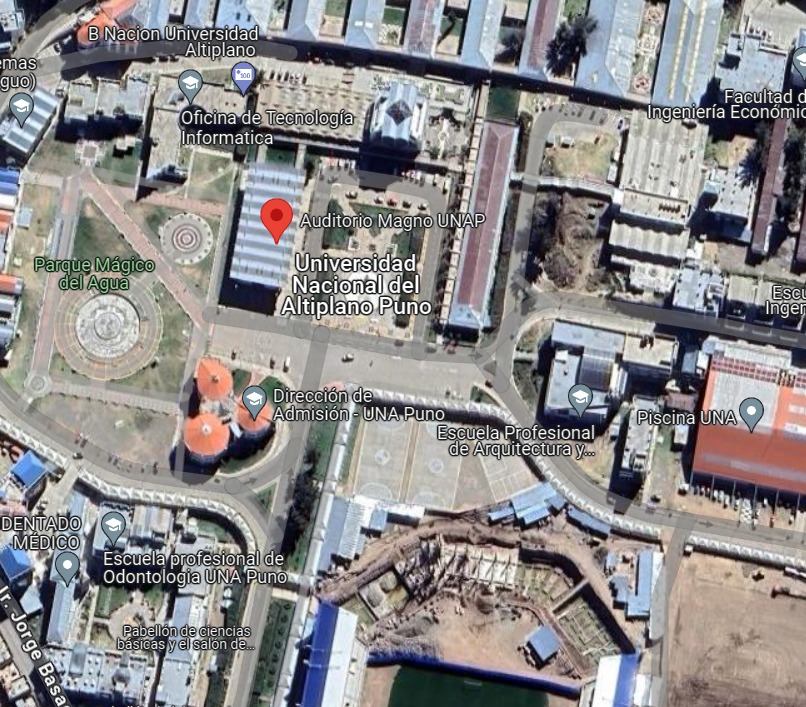
\includegraphics[width=0.7\textwidth]{images/ubicacion.png}
    \caption{Ubicación vista MAPS } \par \textit{Imagen descargada de Google maps}

\end{figure}


\newpage
\section{II. INTRODUCCIÓN DE LA AUDITORÍA}
\subsection*{Dirección de Proyección Social y Extensión Cultural (DPSEC)}

La organización a la cual se realizará la auditoría es un órgano dependiente del Vicerrectorado Académico de la universidad. Ubicada en el campus universitario principal, es responsable de promover, organizar, dirigir y supervisar las actividades en el marco del desarrollo sostenible de Proyección Social y Extensión Cultural, orientadas hacia la comunidad, con el fin de coadyuvar al desarrollo de la región, revalorando la identidad cultural.
\espacio
La DPSEC cuenta con su propio reglamento interno, que establece los derechos y deberes de los participantes y colaboradores. Su infraestructura moderna incluye todos los servicios básicos, oficinas administrativas, salas de reuniones, auditorios para eventos culturales, y áreas destinadas a la interacción comunitaria.

\newpage
\section{III. OBJETIVOS DE LA AUDITORÍA}
\subsection{Definición de objetivo}
Un objetivo es una meta o propósito específico que una persona u organización se propone alcanzar en un plazo determinado.
\\
Metas: Fines específicos de la auditoría.
\\
Plazo: Los términos en unidades de tiempo en que se satisface el fin que se
pretende con la auditoría.


\subsection*{Objetivo general}
Evaluar y asegurar la efectividad de las políticas, procedimientos y prácticas de seguridad de la Dirección de Proyección Social y Extensión Cultural (DPSEC) para garantizar la protección de los recursos humanos, físicos y de información, contribuyendo al cumplimiento de sus objetivos institucionales y al desarrollo sostenible de la Universidad asi mismo recomendar algunas soluciones que beneficie a la organización.

\subsection*{Objetivos específicos}
\subsubsection*{Revisar Políticas y Procedimientos de Seguridad} Evaluar la existencia, adecuación y cumplimiento de las políticas y procedimientos de seguridad establecidos por la DPSEC.

\subsubsection*{Identificar Riesgos y Vulnerabilidades} Detectar posibles riesgos y vulnerabilidades en los sistemas de seguridad física, de la información y de las operaciones diarias.

\subsubsection*{Evaluar la Efectividad de los Controles de Seguridad} Analizar la efectividad de los controles de seguridad implementados para proteger los activos físicos y digitales de la organización.

\subsubsection*{Revisar la Gestión de Incidentes de Seguridad} Evaluar los procedimientos de gestión y respuesta ante incidentes de seguridad, así como la capacidad de la DPSEC para reaccionar y recuperarse de eventos adversos.

\subsubsection*{Verificar la Capacitación y Concientización en Seguridad} Comprobar que el personal de la DPSEC recibe la capacitación adecuada y está concientizado sobre las políticas y procedimientos de seguridad.

\subsubsection*{Recomendar Mejoras y Acciones Correctivas} Proponer mejoras y acciones correctivas para fortalecer el sistema de seguridad de la DPSEC, basadas en los hallazgos de la auditoría.

\subsubsection*{Evaluar el Cumplimiento Normativo} Verificar que la DPSEC cumpla con las normativas y regulaciones aplicables en materia de seguridad.

\newpage
\section{IV. Visita Preliminar}
\subsection{¿Cómo se encuentran distribuidos los sistemas en el área?}
Abarca toda el área de la oficina teniendo el área de trabajos, área de redes, área de recepción y el área de la dirección.
\begin{figure}[!htb]
    \centering
    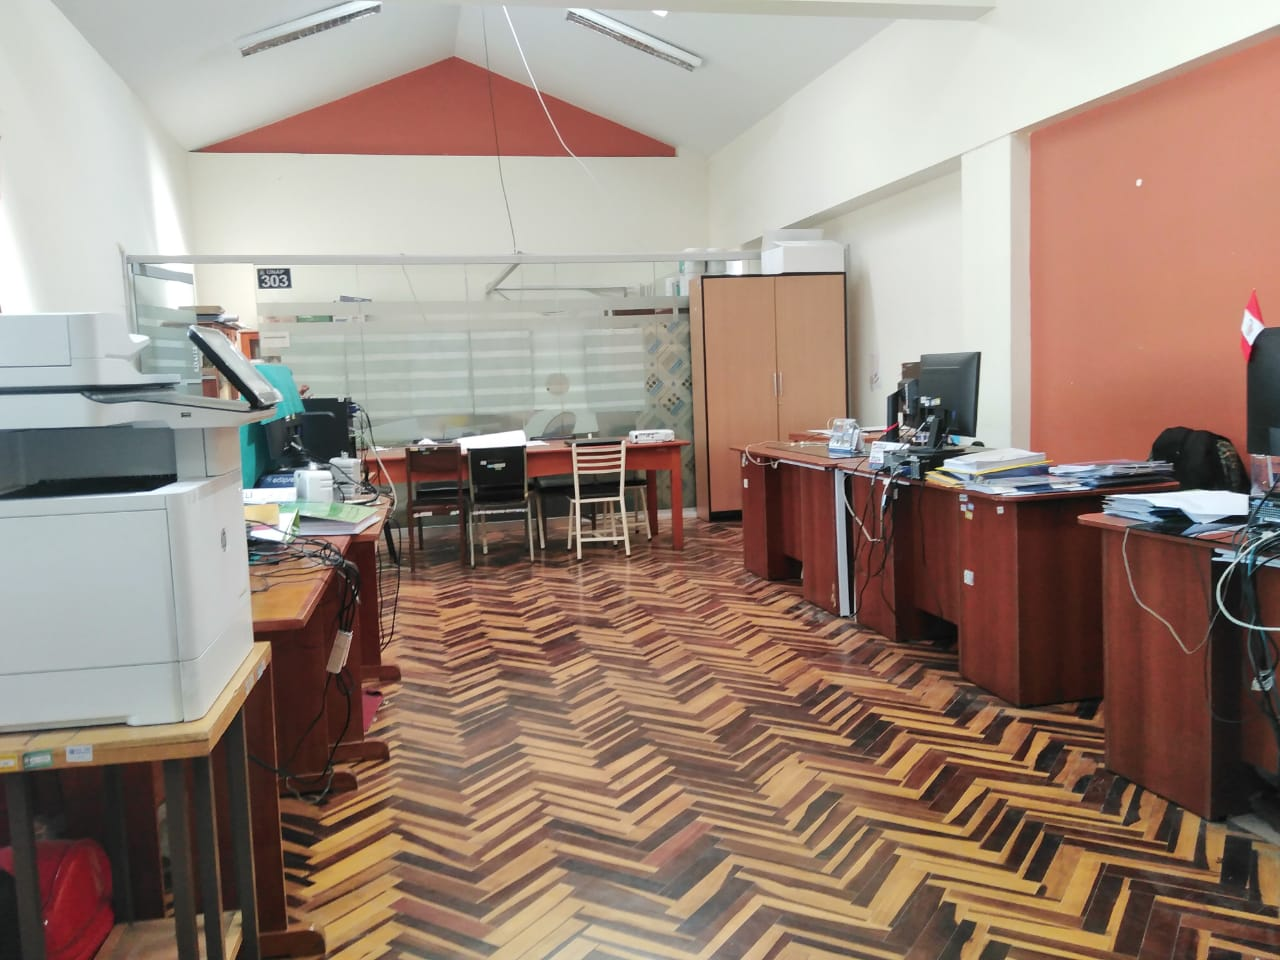
\includegraphics[width=0.7\textwidth]{images/AreaTrabajo.jpeg}
    \caption{Imagen al interior de la dpsec}

\end{figure}

\FloatBarrier

\subsection*{¿Cuántos, cuáles, cómo y de qué tipo son los equipos que están instalados
en el centro de sistemas?}
7 en funcionamiento dentro del área de trabajo de un total de 8 (en total son 6 equipos de computo)
\begin{figure}[!htb]
    \centering
    \animategraphics[autoplay,controls,loop,width=0.4\textwidth]{0.5}{images/equipo}{1}{4}
    \caption{Equipos de la dpsec en total}
\end{figure}
\FloatBarrier
\begin{figure}[!htb]
    \centering
    \animategraphics[autoplay,loop,width=0.4\textwidth]{0.5}{images/datos}{1}{3}
    \caption{Información de la información que maneja}
\end{figure}
\FloatBarrier

\subsection*{¿Qué tipo de instalaciones y conexiones físicas hay en el área de sistemas, y
cómo están distribuidas?}
Cableado  para la fuente de energía, también para los puntos de acceso a internet, cableado en el techo y los cableados para las computadoras.

\begin{figure}[!htb]
    \centering
    \animategraphics[autoplay,controls,loop,width=0.4\textwidth]{0.5}{images/fisica}{1}{4}
    \caption{instalaciones físicas de cable}
\end{figure}

\newpage
\subsubsection*{Contacto Inicial}
Observe su reacción al llevar el documento de solicitud para realizar la auditoria un miedo a que no me proporcionaran dicha información 
que yo necesitaría sim embargo la respuesta fue algo similar pero que resultados positivos me acepto pero nos dijeron que nosotros tenemos que presentar un documento 
especialmente como ellos quieren para fortalecer los puntos débiles encontrada por nosotros los auditores.
\begin{figure}[!htb]
    \centering
    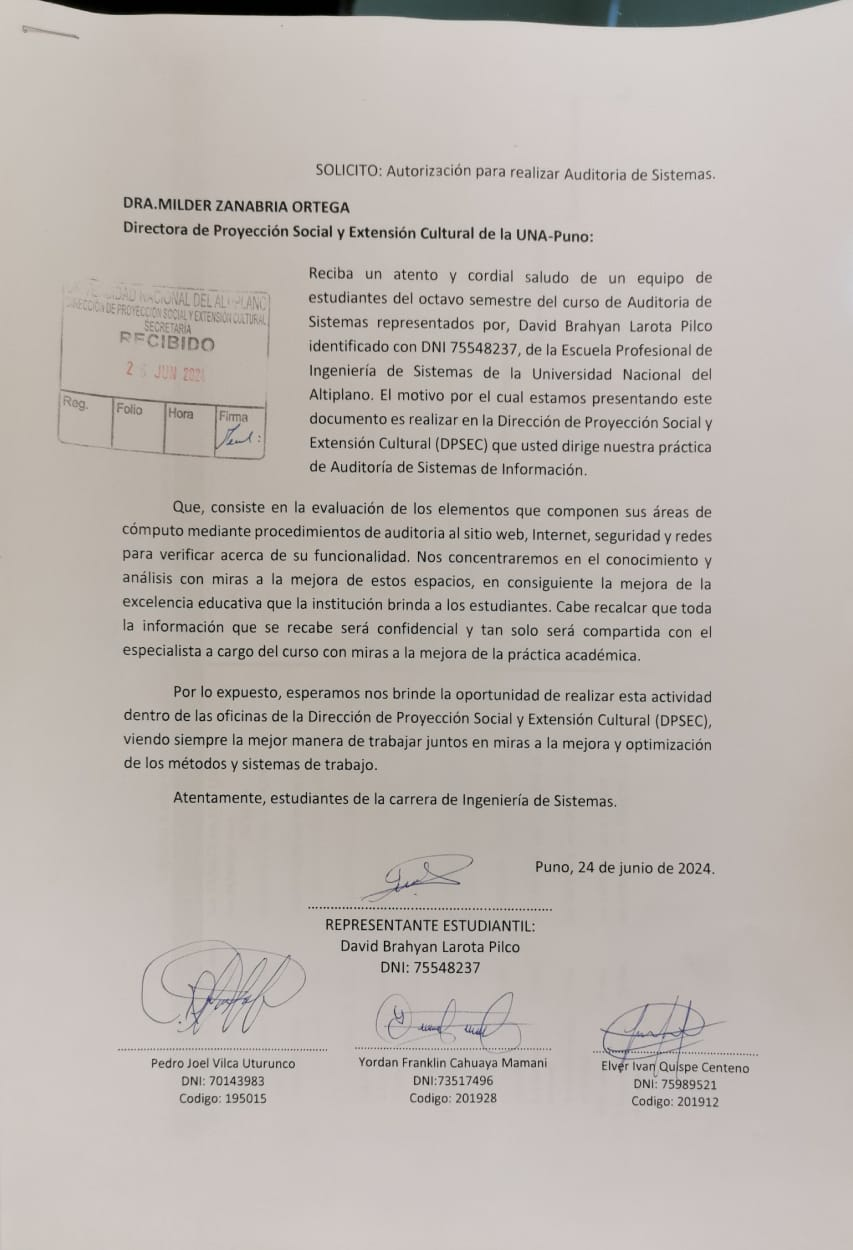
\includegraphics[width=0.4\textwidth]{images/solicitud.jpeg}
    \caption{foto de evidencia Solicitud }

\end{figure}

\subsection*{¿Cómo reacciona el personal ante la visita del auditor? ¿Cuáles son las
medidas de seguridad visibles que existen?}
El personal encargado de nuestra visita era una egresada de la carrera de ingeniera de sistemas
nos ayudo en muchas cosas nos explico y corrigió en algunos aspectos cabe recalcar que el personal era
un egresado de mucho tiempo y se mostró una actitud de querer volver a aprender sobre la auditoria.
Pero nos mostró cada área cada petición que le pedimos nos dijo tal cual.

\newpage
\section{V. ORGANIGRAMA DE LA ORGANIZACIÓN}
\begin{figure}[!htb]
    \centering
    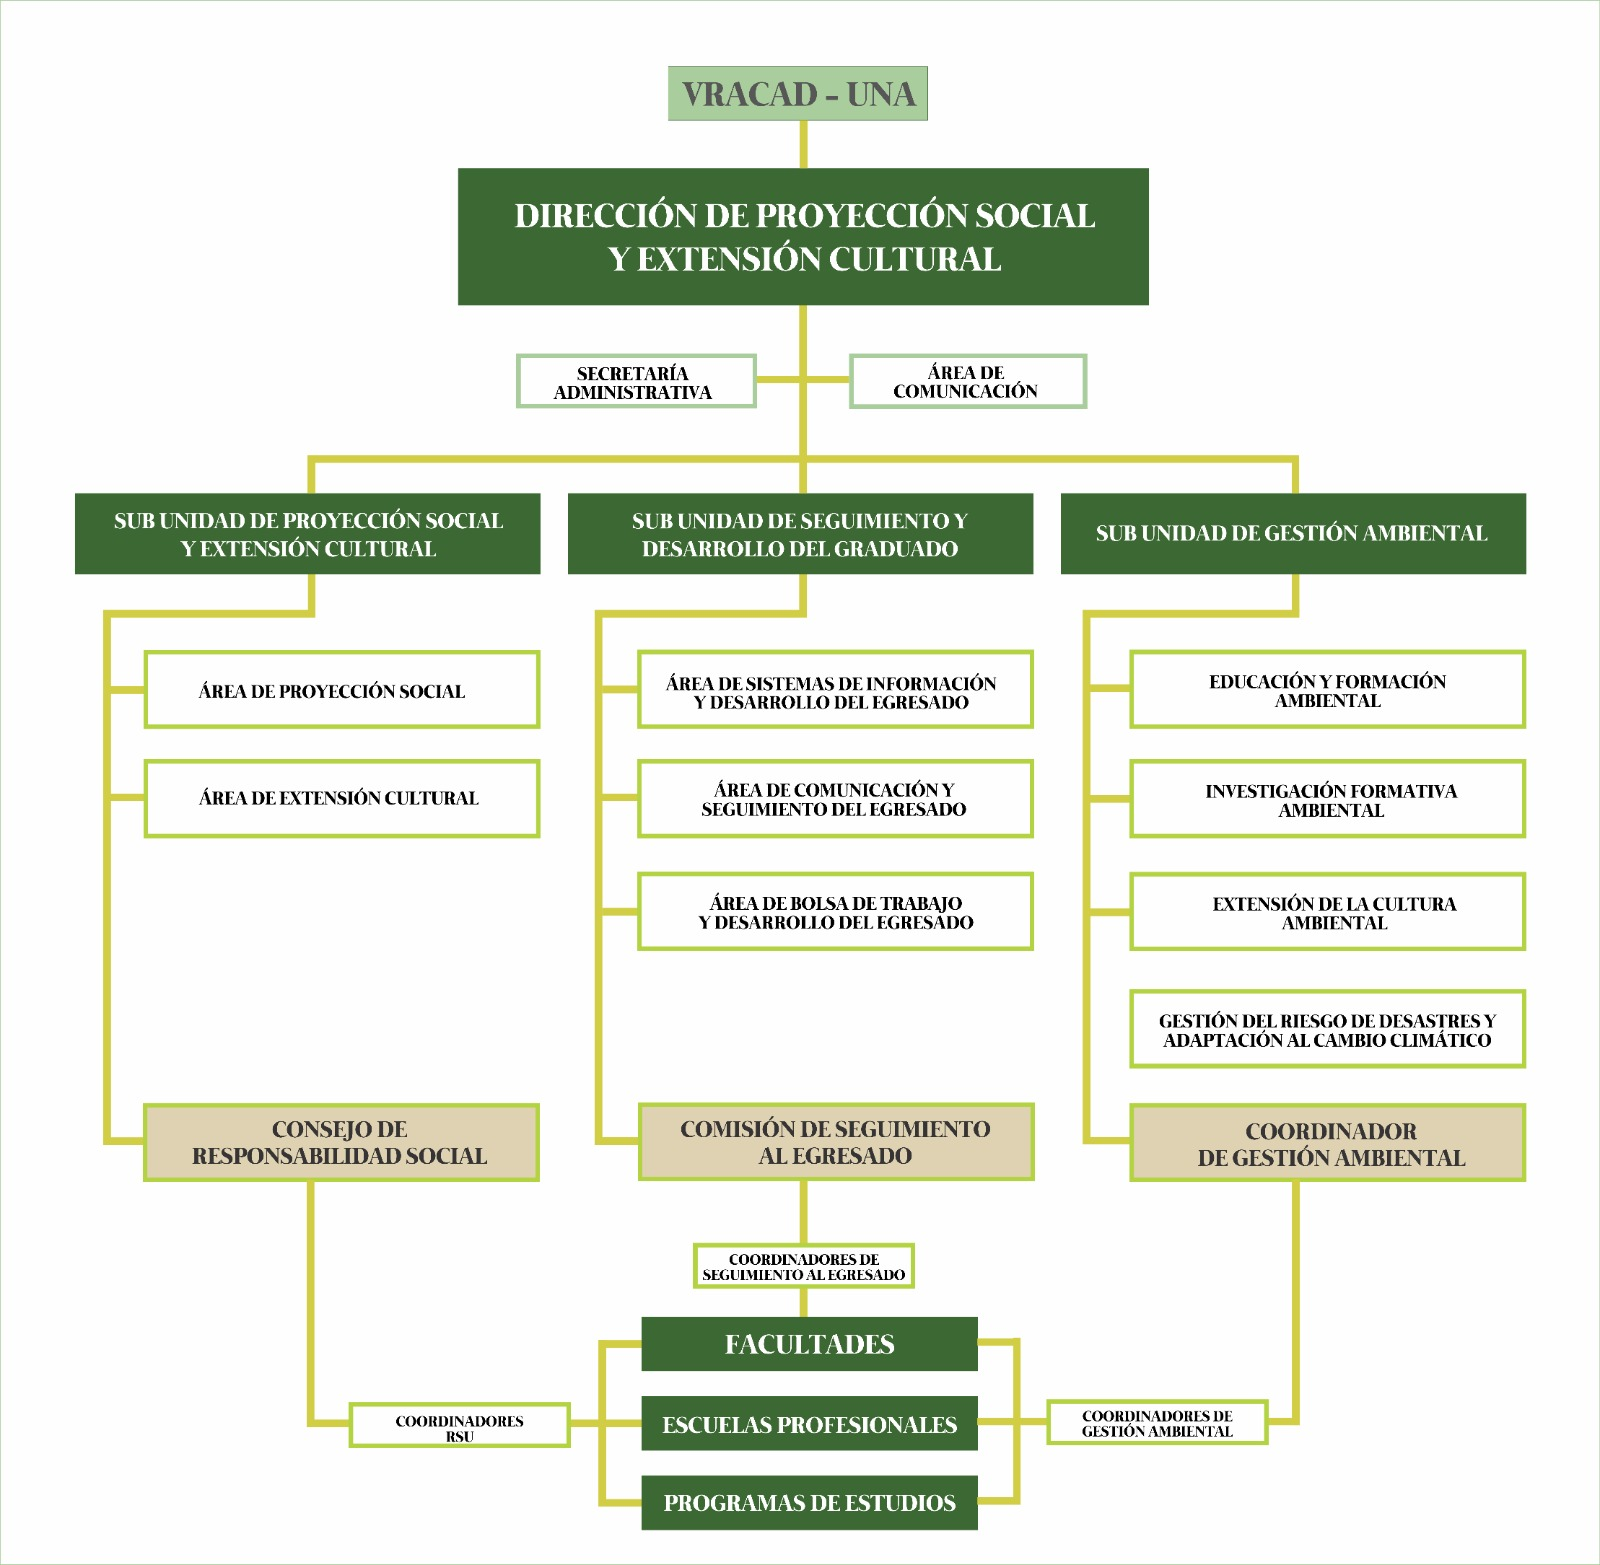
\includegraphics[width=0.6\textwidth]{images/organigrama.jpeg}
    \caption{organigrama de la organización}

\end{figure}

\newpage
\section{VI. ÁREAS A SER AUDITADAS DE LA ORGANIZACIÓN}
El área principal donde esta la oficina principal solo tiene un área, asi que específicamente auditare en la Dirección de Proyección Social y Extensión Cultural (DPSEC) en términos de seguridad son las siguientes:
\begin{figure}[!htb]
    \centering
    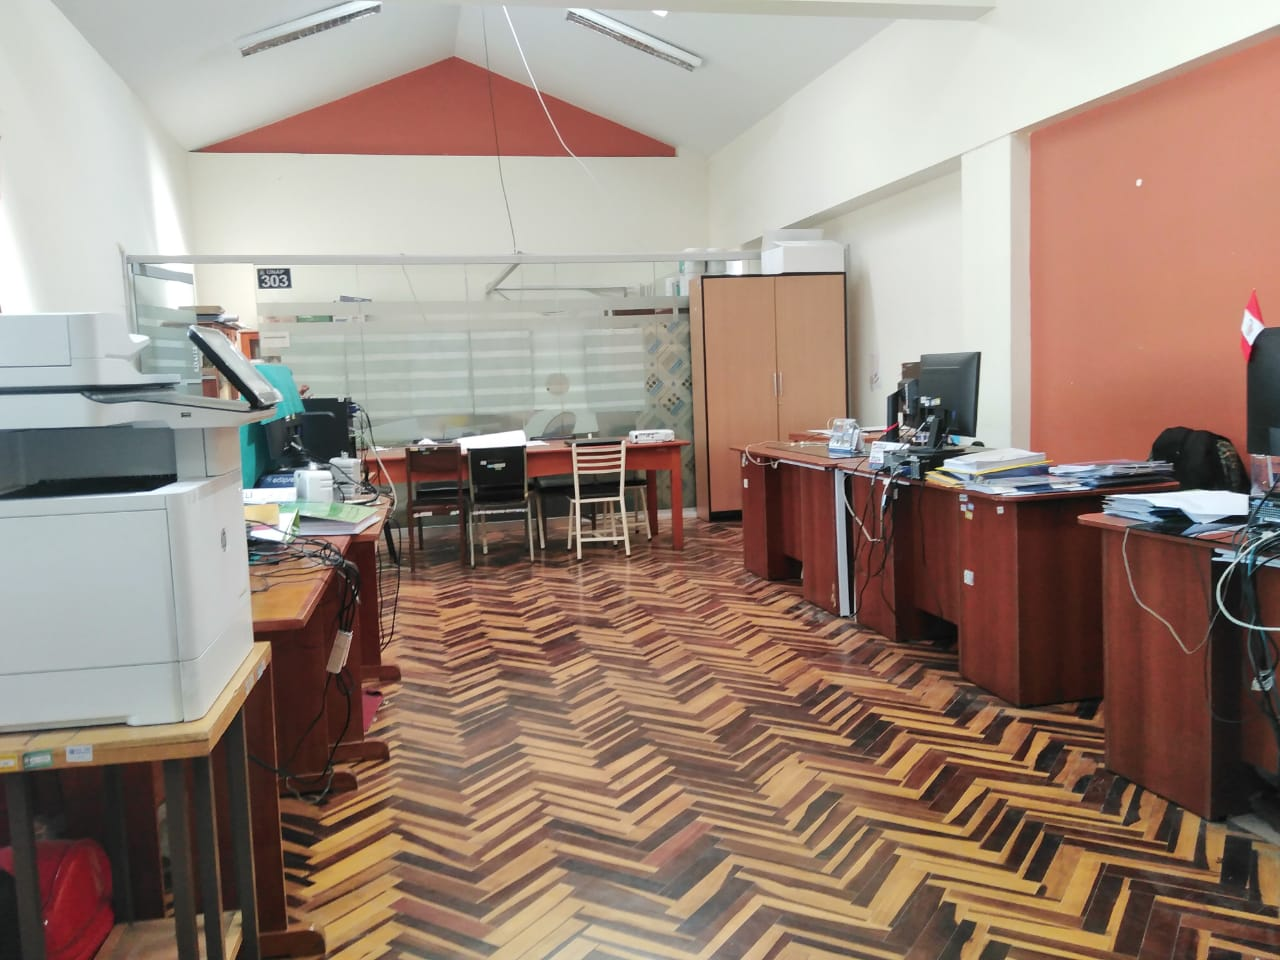
\includegraphics[width=0.6\textwidth]{images/AreaTrabajo.jpeg}
    \caption{Área donde esta todo en un ambiente. Como al fondo podemos ver el área de redes}
    
\end{figure}
\begin{itemize}
    \item \textbf{Políticas y Procedimientos de Seguridad:} Revisión y evaluación de las políticas y procedimientos de seguridad existentes, asegurando que estén documentados, actualizados y se cumplan adecuadamente.
    \item \textbf{Gestión de Riesgos y Vulnerabilidades:} Identificación y análisis de los riesgos y vulnerabilidades que pueden afectar la seguridad física, de la información y operativa de la DPSEC.
    \item \textbf{Controles de Seguridad:} Evaluación de la efectividad de los controles de seguridad implementados para proteger los activos físicos y digitales, incluyendo acceso físico a instalaciones y medidas de ciberseguridad.
    \item \textbf{Gestión de Incidentes de Seguridad:} Revisión de los procedimientos y protocolos para la gestión y respuesta ante incidentes de seguridad, así como la capacidad de recuperación ante eventos adversos.
    \item \textbf{Capacitación y Concientización en Seguridad:} Verificación de los programas de capacitación y concientización en seguridad destinados al personal de la DPSEC, asegurando que todos los empleados conozcan y cumplan con las políticas y procedimientos de seguridad.
    \item \textbf{Cumplimiento Normativo:} Evaluación del cumplimiento de la DPSEC con las normativas y regulaciones aplicables en materia de seguridad.
    \item \textbf{Infraestructura y Equipamiento de Seguridad:} Inspección de la infraestructura y el equipamiento de seguridad disponibles, como cámaras de vigilancia, sistemas de alarma, controles de acceso, entre otros.
    
\end{itemize}

\newpage
\section{VII. TIPO DE AUDITORÍA A UTILIZAR}
\subsection{Auditoria de la seguridad de los sistemas computacionales}
Dada la estructura de la organización DPSEC, donde todos los equipos de cómputo y redes se encuentran centralizados en un único área, es crucial garantizar la integridad, disponibilidad y confidencialidad de los sistemas. 
Esta auditoría de seguridad permitirá identificar vulnerabilidades, evaluar riesgos y asegurar que se implementen las mejores prácticas de protección de la información y los activos tecnológicos. 
Además, ayudará a cumplir con las normativas y estándares de seguridad, asegurando la continuidad operativa y la confianza de la Universidad y partes interesadas.
\begin{figure}[!htb]
    \centering
    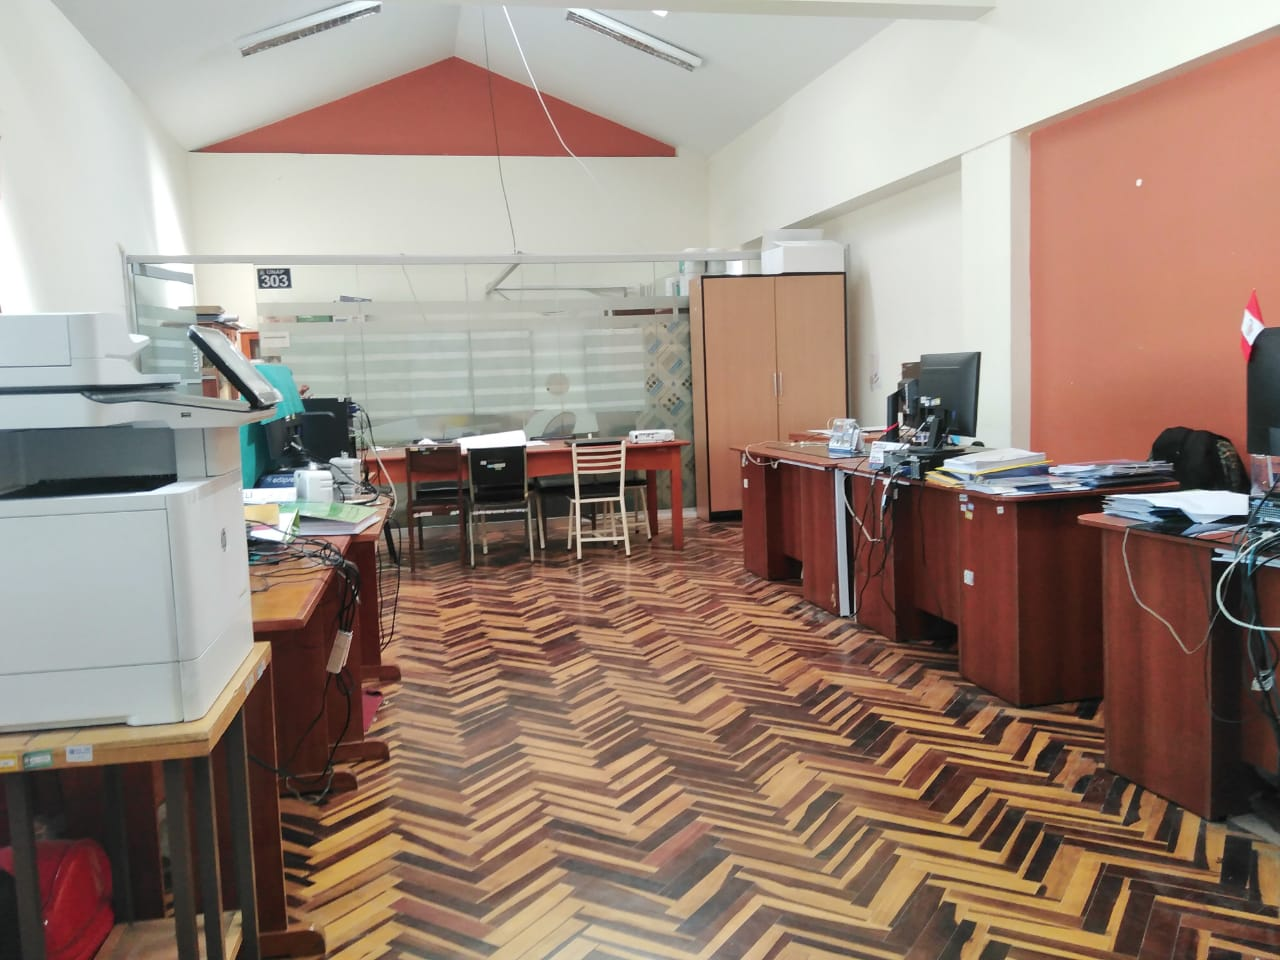
\includegraphics[width=0.6\textwidth]{images/AreaTrabajo.jpeg}
    \caption{Área de la dpsec}
    
\end{figure}

\newpage
\section{VIII. INSTRUMENTOS DE AUDITORÍA}
Los instrumentos y herramientas de auditoría que utilizará y justificar la importancia que
este tendrá en la Auditoría.
\subsection{Recopilación y análisis de la información}
\subsubsection{Entrevistas}
Al personal que se encuentre relacionado con la seguridad.
\subsection{La observación}
Visitas preliminares
Ubicación geográfica 
\subsection{Las pruebas y simulaciones de los sistemas}

\begin{table}[ht]
    \centering
    \caption{Recursos informáticos }
    \begin{tabular}{cc}
        \toprule
        Área & Software a usar para Auditar \\
        \midrule
        Seguridad de la información  & ISO/IEC 27001:2013 \\
        Redes.  & Nessus\\
        Seguridad física & Metasploit \\        \bottomrule
    \end{tabular}
    
\end{table}

\newpage
\section{IX PERSONAL PARA LA AUDITORÍA}
\begin{figure}[!htb]
    \centering
    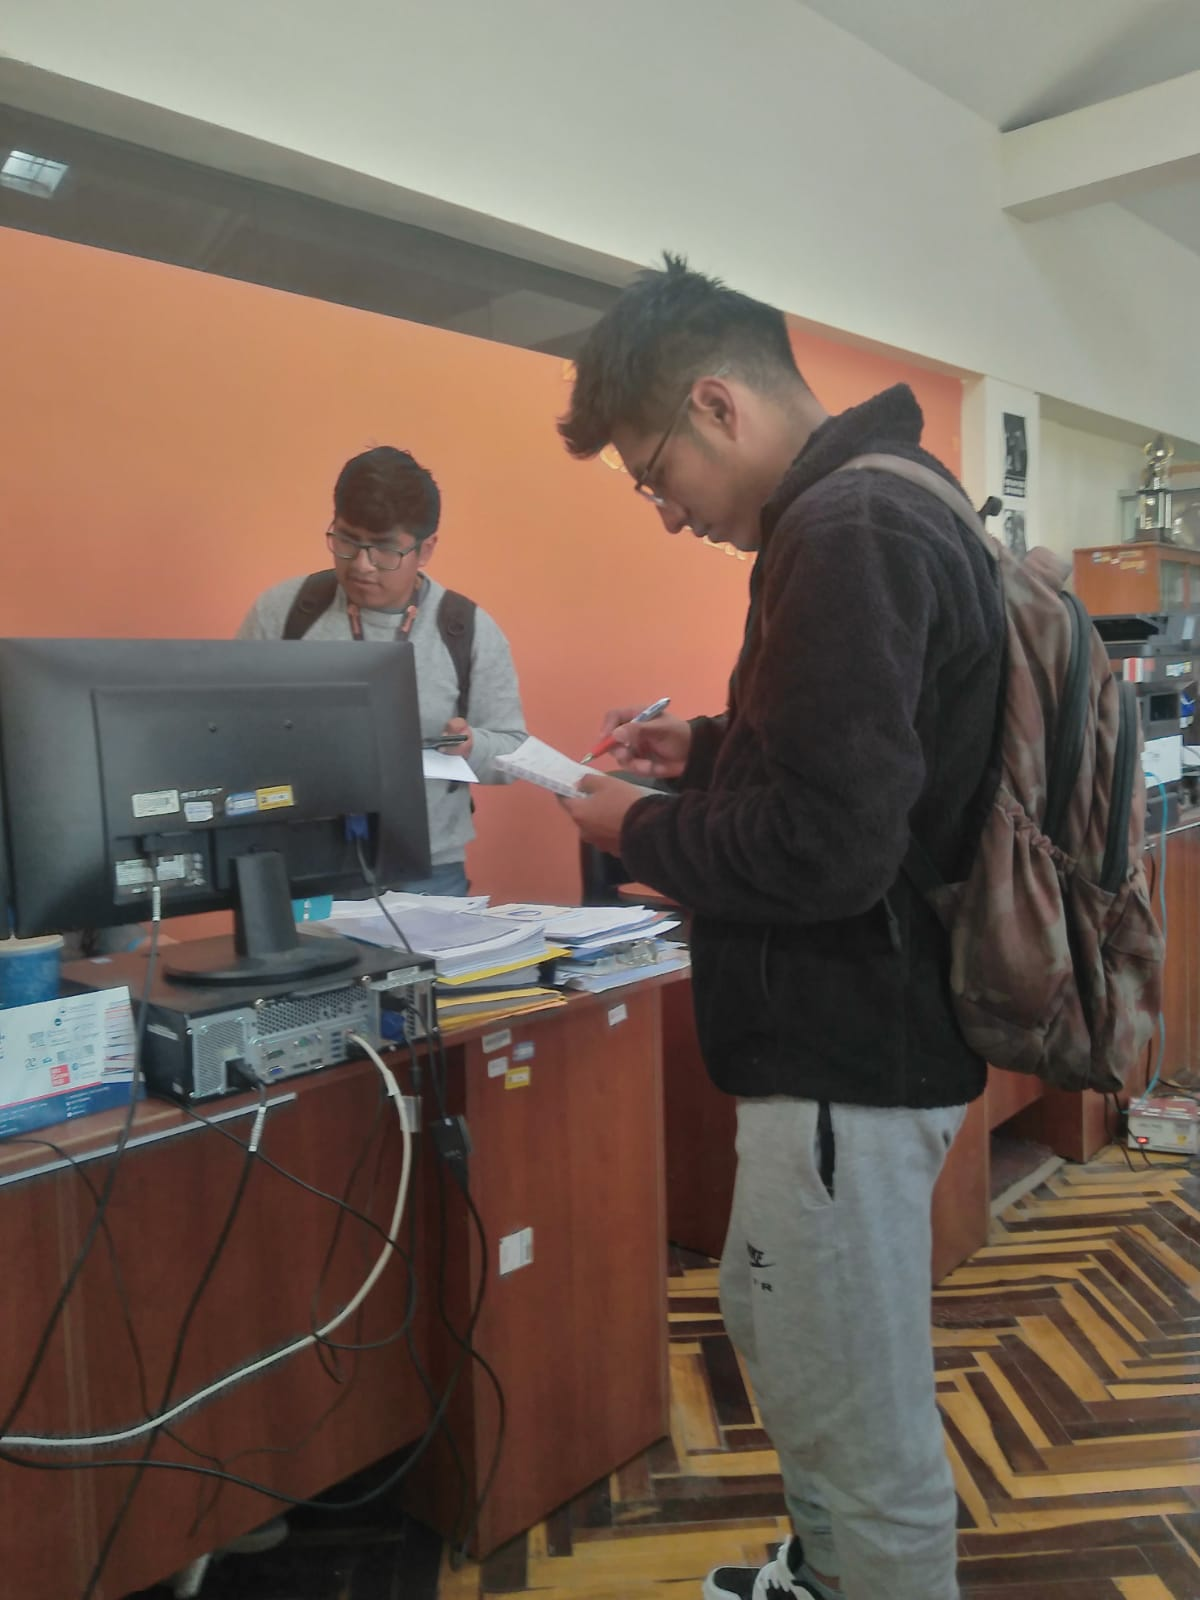
\includegraphics[width=0.6\textwidth]{images/evidencia.jpeg}
    \caption{Evidencia de la Auditoria}
    
\end{figure}

\section*{PERSONAL PARA LA AUDITORÍA}
\subsection*{Funciones en común de todo el personal}
\begin{itemize}
    \item Visita preliminar a la organización.
    \item Realizar entrevistas a los encargados de la organización.
    \item Realizar las auditorías con las herramientas preestablecidas.
    
\end{itemize}

\begin{table}[ht]
    \centering
    \begin{tabular}{cc}
        \toprule
        \textbf{Foto} & \textbf{Nombre del Auditor} \\
        \midrule
        
        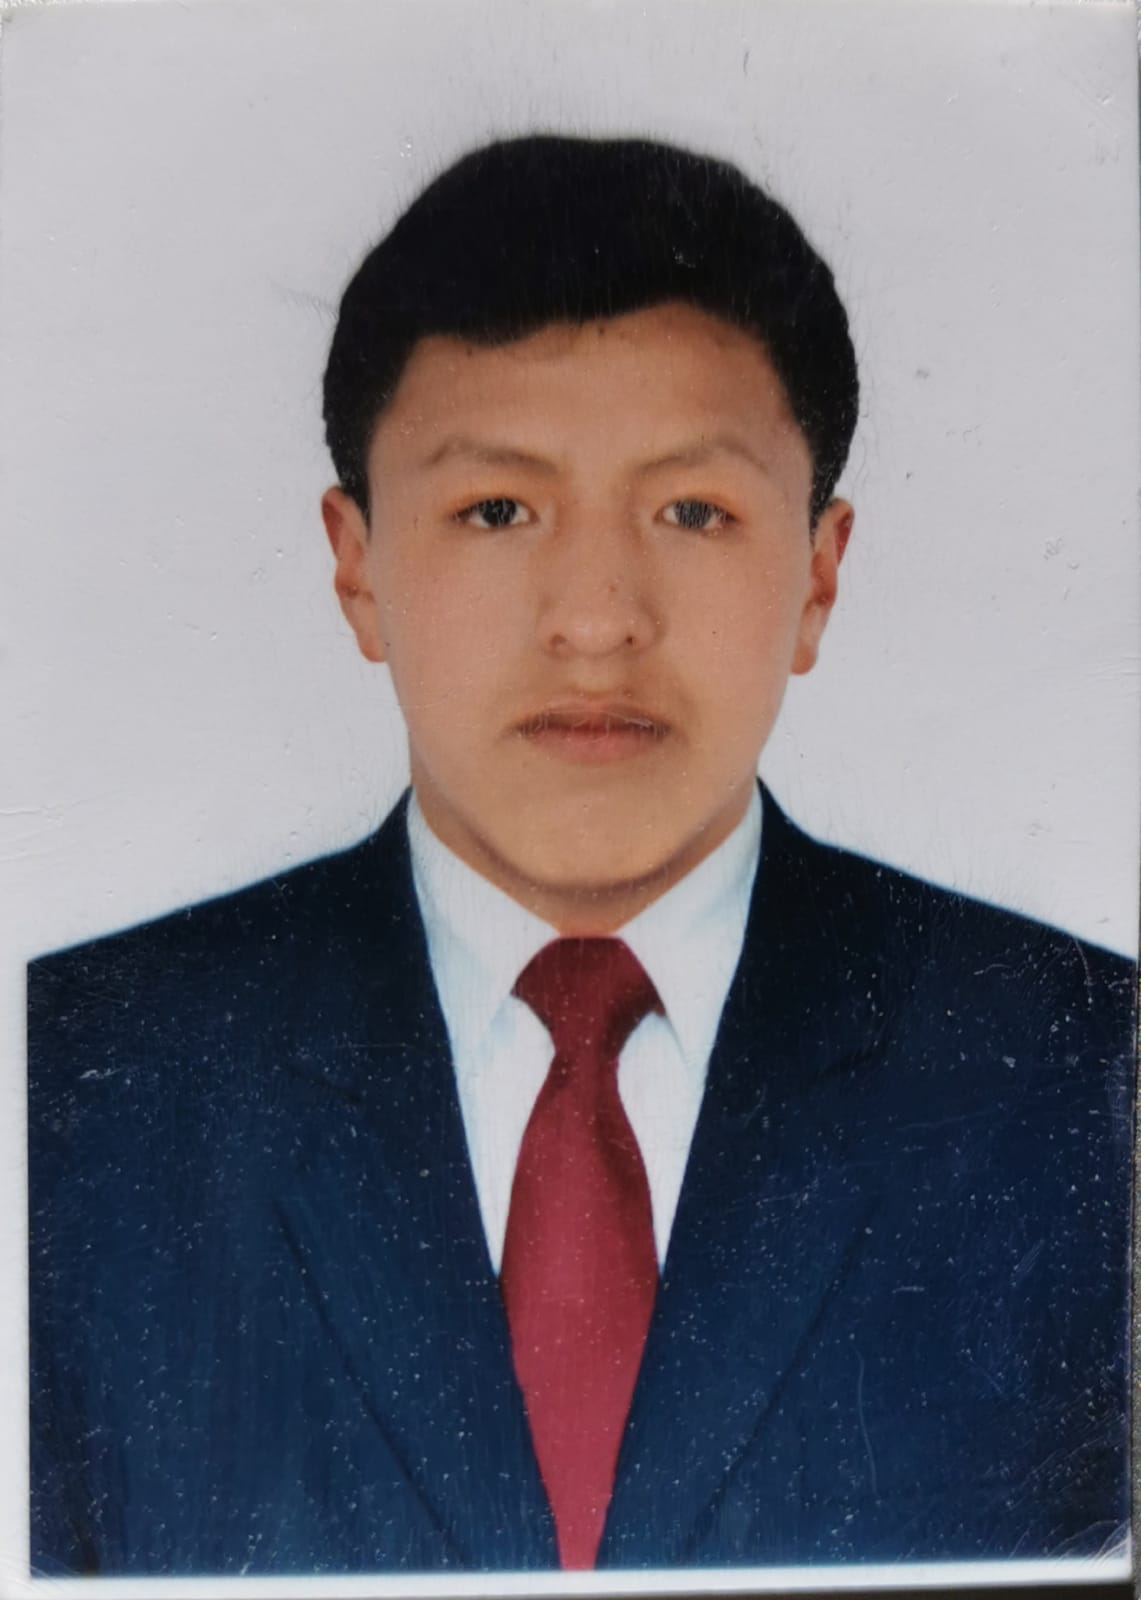
\includegraphics[width=0.17\textwidth]{images/fotodavid.jpeg} & David Brahyan Larota Pilco \\
        
        \bottomrule
    \end{tabular}
    \caption{Foto del primer Auditor}
    \par \textbf{Funciones} \par Examinar la información y los antecedentes de la organización. \\
    Velar por la precisión y consistencia de la información.
    
\end{table}

\newpage
\section{X GESTIÓN DEL TIEMPO DE PROYECTO}
Se muestra el avance del Proyecto y los días designados.
\begin{figure}[!htb]
    \centering
    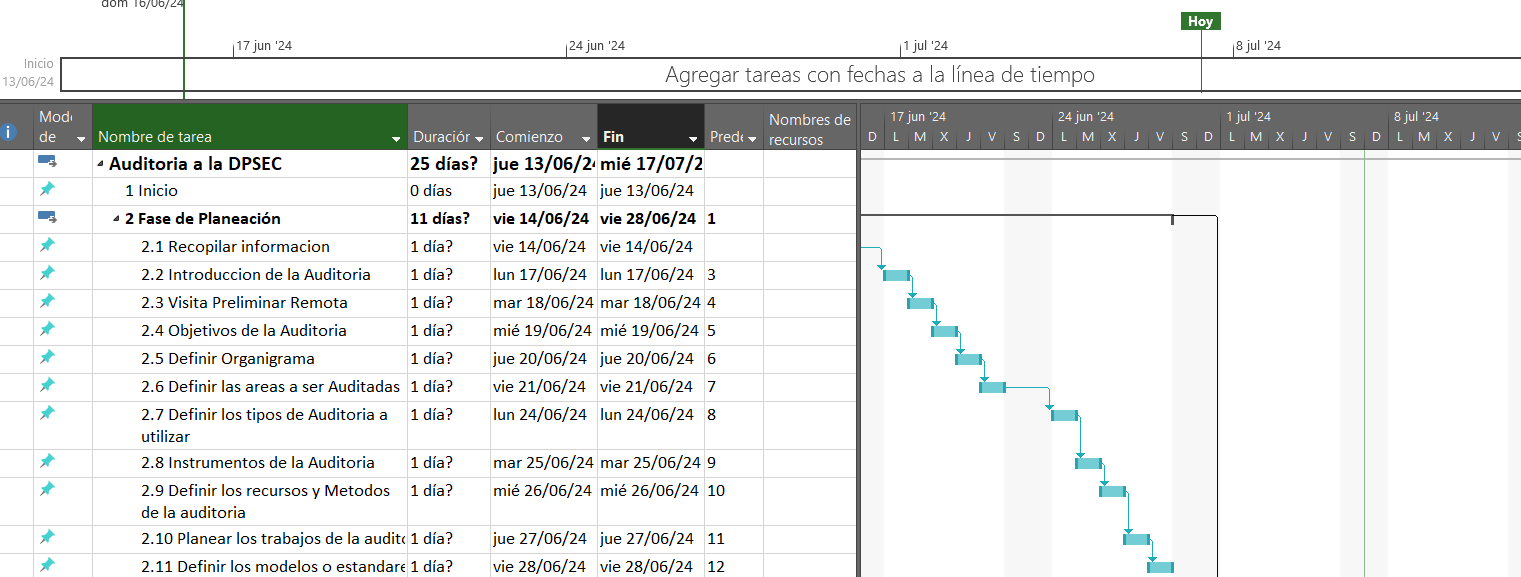
\includegraphics[width=0.8\textwidth]{images/cronograma1.png}
    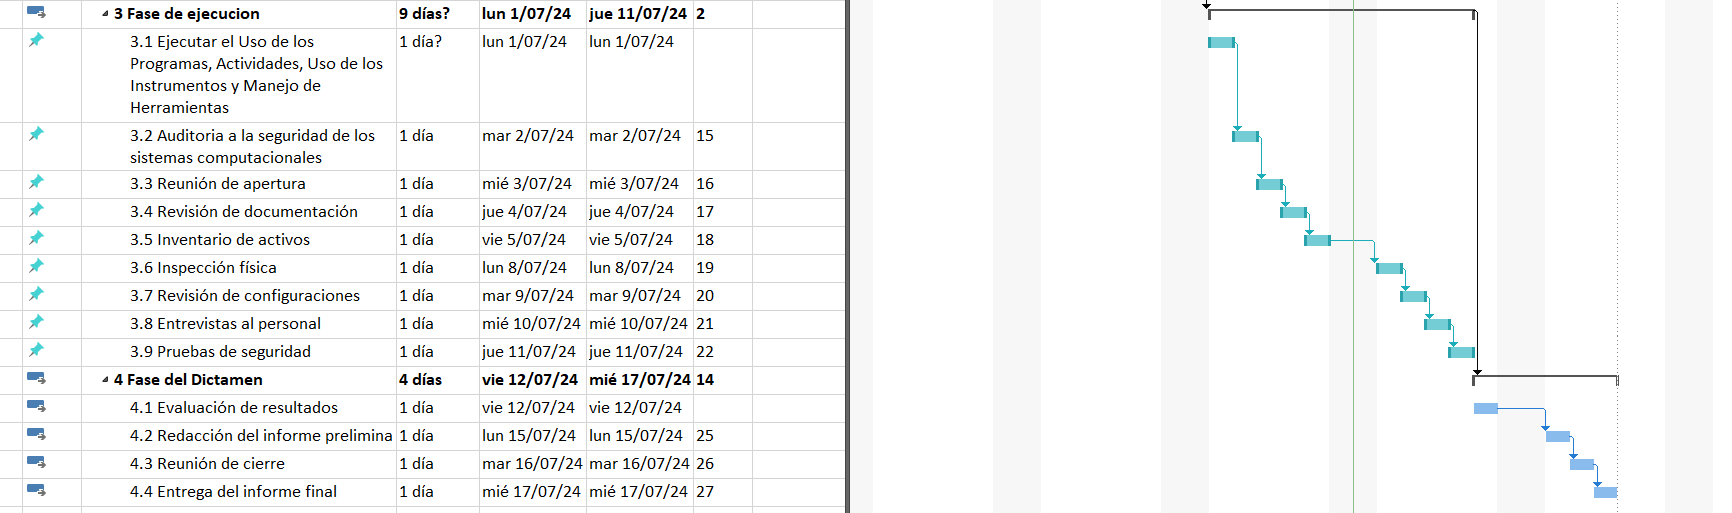
\includegraphics[width=0.8\textwidth]{images/cronograma2.png}
    \caption{Fotos del cronograma}
    
\end{figure}

\newpage
\section{XI PLANES DE TRABAJO O PROGRAMAS DE LA AUDITORÍA}
Planes de trabajo o programas de la auditoría\\
Se está desarrollando los planes o programas de auditoría de cada acción y actividad que
se está teniendo en el proyecto de auditoría de la entidad “DPSEC”
como son:

\begin{figure}[!htb]
    \centering
    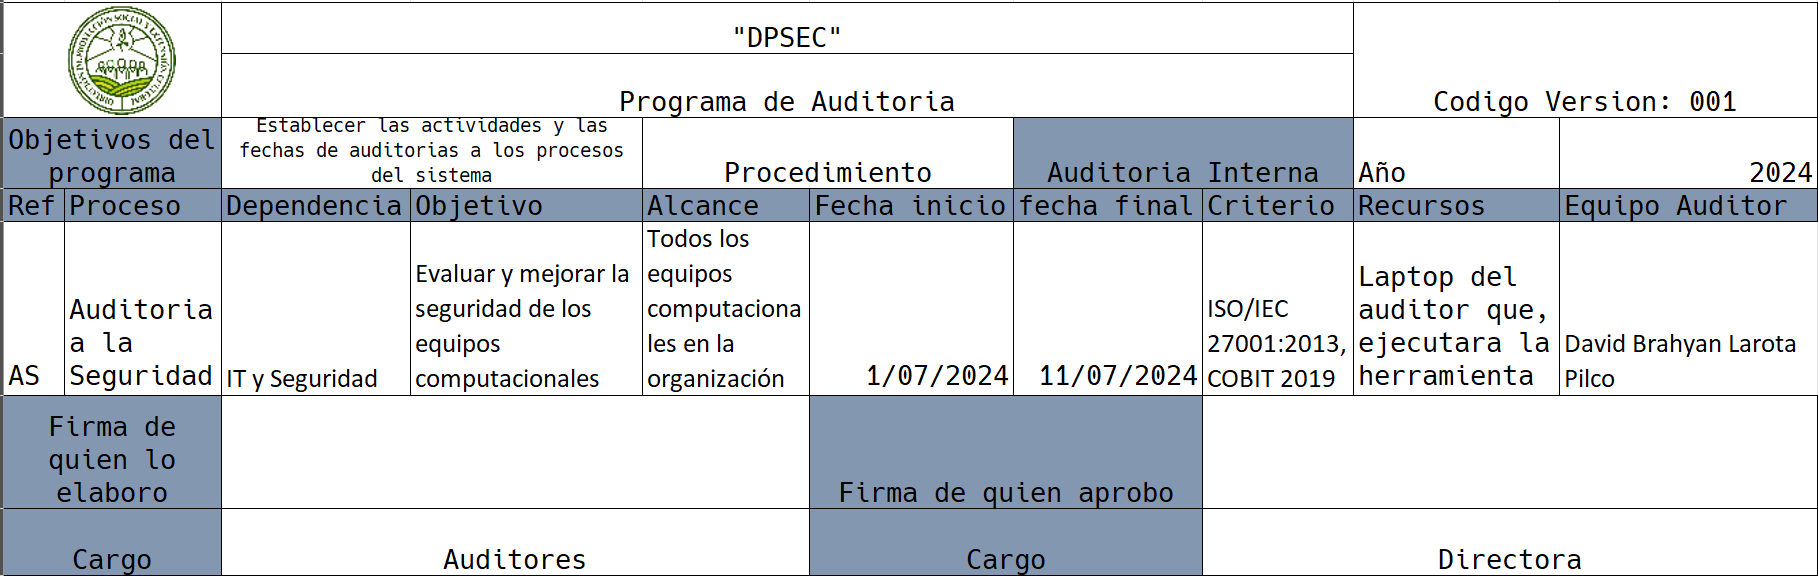
\includegraphics[width=0.8\textwidth]{images/planTrabajo.png}
    \caption{Plan de Trabajo}
    
\end{figure}
\FloatBarrier
\begin{figure}[!htb]
    \centering
    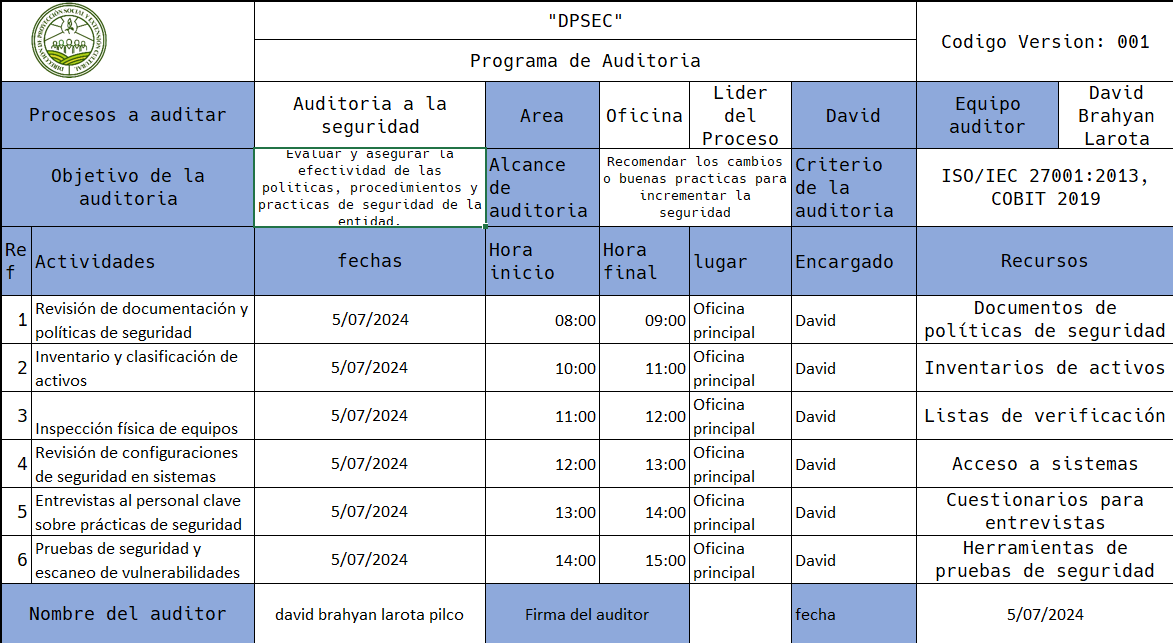
\includegraphics[width=0.8\textwidth]{images/planEjecucion.png}
    \caption{Plan de Trabajo para la Auditoria de Seguridad}
    
\end{figure}
Se está desarrollando el modelo de los instrumentos a utilizar en la auditoría y desarrollar una
descripción de la importancia de este instrumento, además si se utiliza algún recurso tecnológico
indicar la importancia que este tendrá y de qué forma ayuda en la auditoría.

\begin{table}[ht]
    \centering
    \begin{tabular}{cc}
        \toprule
        \textbf{Tipo de Recurso} & \textbf{Herramienta} \\
        \midrule
        Material  &  Cámara Fotográfica ,Grabadora de audio  \\
        Técnico   & Papeles de trabajo, Lapiceros \\
        Económico &  Pasajes, Alimentación \\
        \bottomrule
    \end{tabular}
    \caption{Tabla recursos y herramientas}
    
\end{table}

\section{XII MODELOS Y ESTÁNDARES DE LA AUDITORÍA}
Se indican los modelos, metodologías, estándares y otros que serán utilizados en la auditoría.
\subsection{Norma Para la seguridad ISO/IEC 27001:2013}
ISO/IEC 27001:2013 es un estándar internacional que describe las mejores prácticas para un sistema de gestión de seguridad de la información (SGSI). Fue desarrollado conjuntamente por la Organización Internacional de Normalización (ISO) y la Comisión Electrotécnica Internacional (IEC).
\subsection*{Qué Proporciona}
\subsection*{Estructura para la Seguridad de la Información}
Proporciona un marco para establecer, implementar, mantener y mejorar continuamente un SGSI.
Ayuda a las organizaciones a proteger sus activos de información mediante la aplicación de un conjunto de controles de seguridad de la información gestionados sistemáticamente.
\subsection*{Gestión de Riesgos}

Incluye la evaluación y el tratamiento de riesgos de seguridad de la información específicos de la organización.
Permite a las organizaciones identificar amenazas, vulnerabilidades y sus impactos, y aplicar controles adecuados para mitigarlos.
\subsection*{Controles de Seguridad}

Proporciona un conjunto de controles de seguridad organizados en 14 dominios que abarcan desde la política de seguridad hasta el cumplimiento legal.
Estos dominios incluyen:
\begin{enumerate}
    \item Políticas de seguridad de la información
    \item Organización de la seguridad de la información
    \item Seguridad de los recursos humanos
    \item Gestión de activos
    \item Control de acceso
    \item Criptografía
    \item Seguridad física y del entorno
    \item Seguridad de las operaciones
    \item Seguridad de las comunicaciones
    \item Adquisición, desarrollo y mantenimiento de sistemas
    \item Relaciones con los proveedores
    \item Gestión de incidentes de seguridad de la información
    \item Aspectos de seguridad de la información en la gestión de la continuidad del negocio
    \item Cumplimiento
    
\end{enumerate}
\subsection*{Cumplimiento y Certificación}

Permite a las organizaciones obtener la certificación de conformidad con el estándar, demostrando a clientes y socios su compromiso con la seguridad de la información.
Facilita el cumplimiento de requisitos legales y regulatorios relacionados con la protección de datos y la seguridad de la información.
\subsection*{Mejora Continua}

Establece un ciclo de mejora continua (Plan-Do-Check-Act, PDCA) para gestionar y mejorar la seguridad de la información de manera sistemática.
Fomenta una cultura de seguridad dentro de la organización, asegurando que las prácticas de seguridad evolucionen con el tiempo.

\newpage
\section{EJECUCIÓN DE LA AUDITORÍA}


EJECUCIÓN DE LOS PROGRAMAS, ACTIVIDADES, IMPLEMENTACIÓN DE LOS INSTRUMENTOS,
HERRAMIENTAS TECNOLÓGICAS

\section{I Procesos}
\subsection{Auditoria a la Seguridad}
\begin{figure}[!htb]
    \centering
    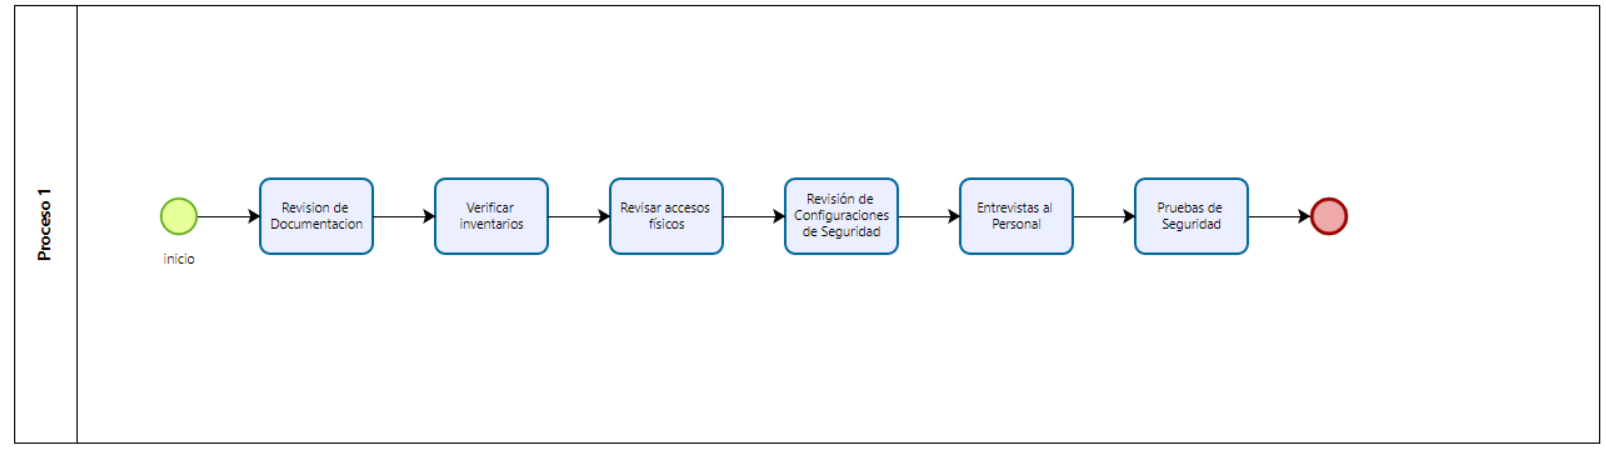
\includegraphics[width=0.8\textwidth]{images/proceso1.png}
    \caption{Proceso para ejecutar la auditoria a la seguridad}
    \par Diagrama realizado en BIZAGI
\end{figure}
\FloatBarrier 

\newpage
\section{II DESARROLLO DE LOS PAPELES DE TRABAJO DE LA AUDITORÍA}
\subsection{Hoja de identificación}
\begin{figure}[!htb]
    \centering
    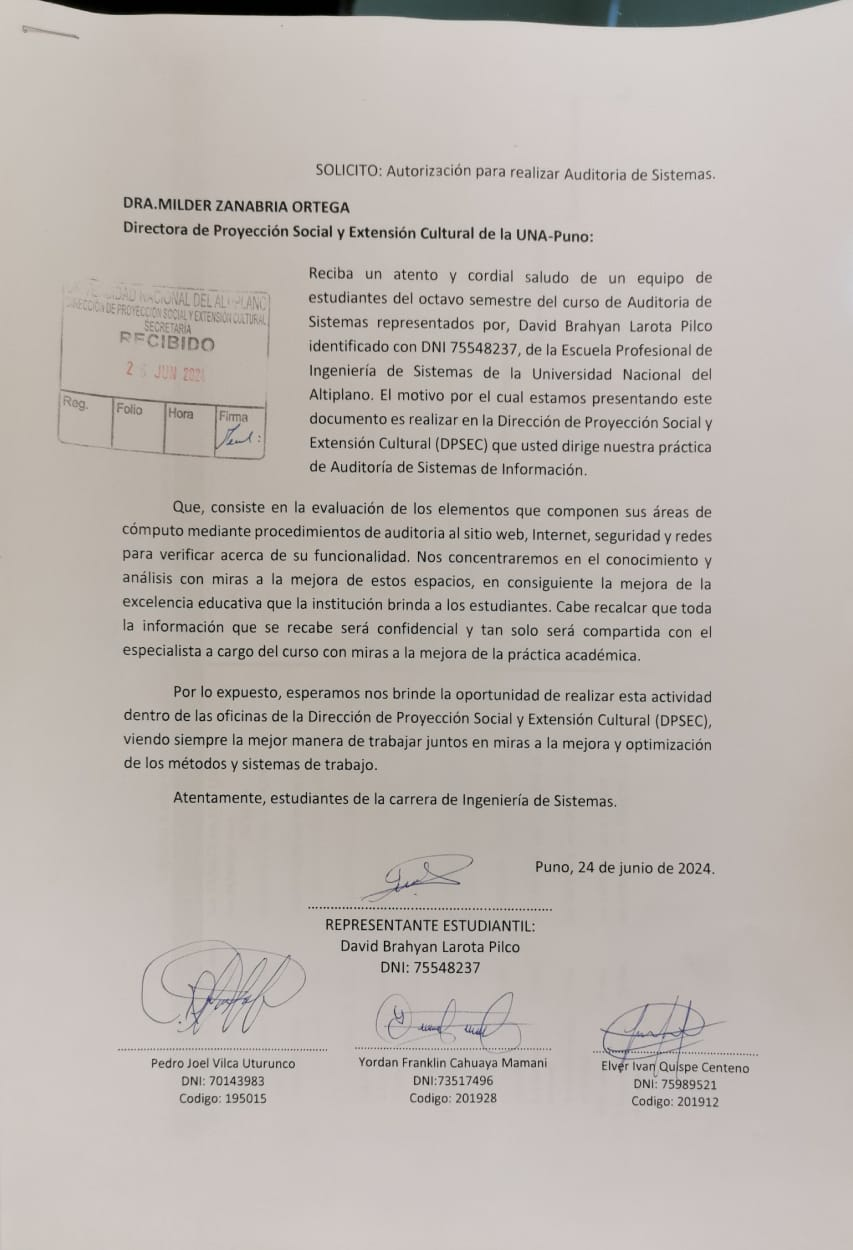
\includegraphics[width=0.7\textwidth]{images/solicitud.jpeg}
    
\end{figure} 
\FloatBarrier 
\subsection{Índice de contenido de los papeles}
\begin{table}[ht]
    \centering
    \begin{tabular}{|c|c|}
        \toprule
        \textbf{AS} & \textbf{Documentación para la Auditoria a la Seguridad} \\
        \bottomrule
    \end{tabular}
    \caption{Tabla recursos y herramientas}
    
\end{table}


\subsection{Resumen de las situaciones encontradas}
\subsubsection*{Desviaciones Relevantes}
\begin{figure}[!htb]
    \centering
    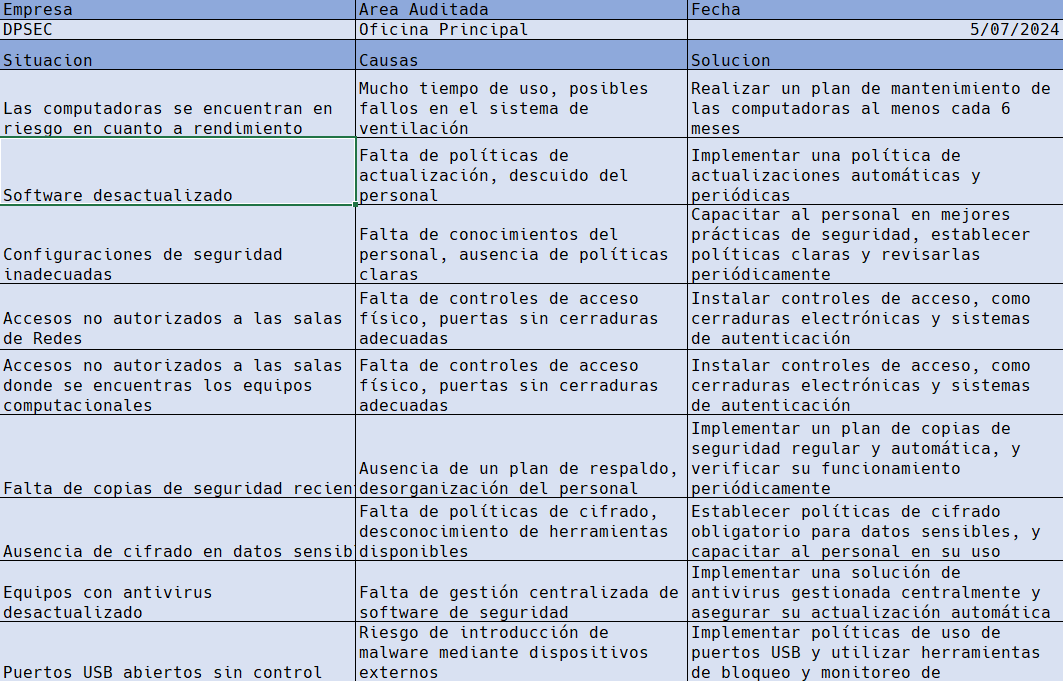
\includegraphics[width=0.8\textwidth]{images/desviaciones.png}
    
\end{figure} 

\subsection{Situaciones encontradas}
\begin{figure}[!htb]
    \centering
    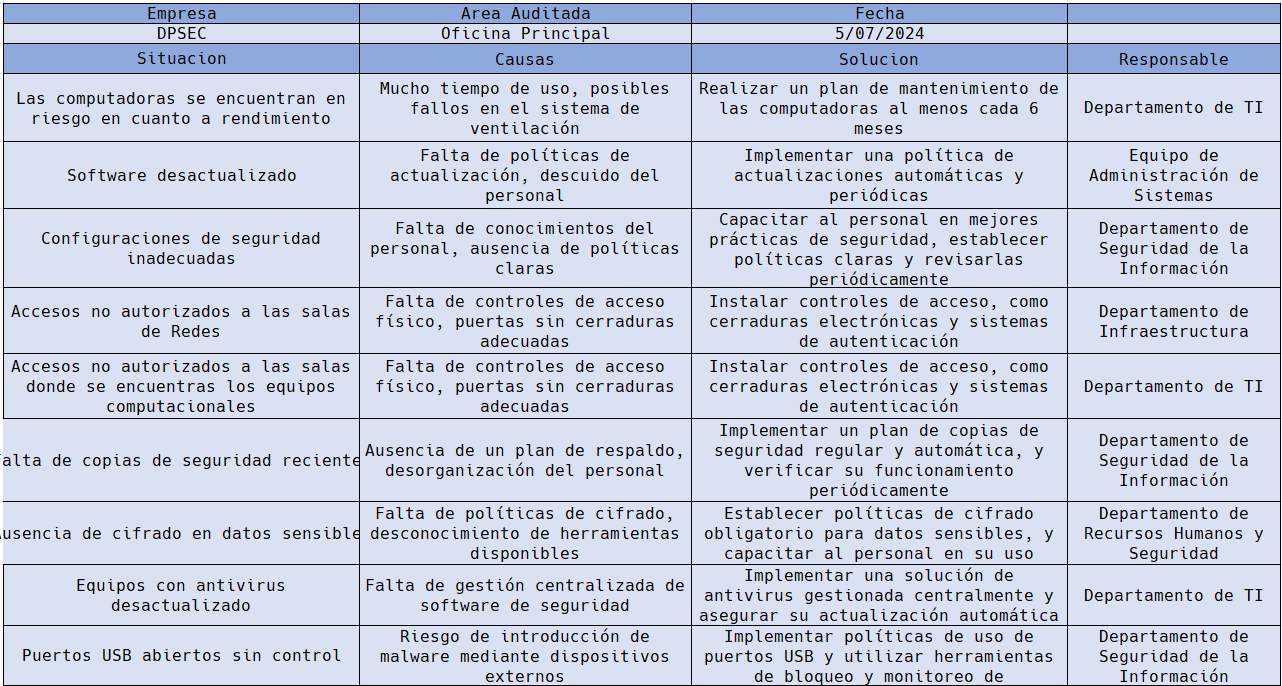
\includegraphics[width=0.8\textwidth]{images/responsable.png}
    
\end{figure} 
\FloatBarrier 

\subsection{Guía de Auditoria }
\begin{figure}[!htb]
    \centering
    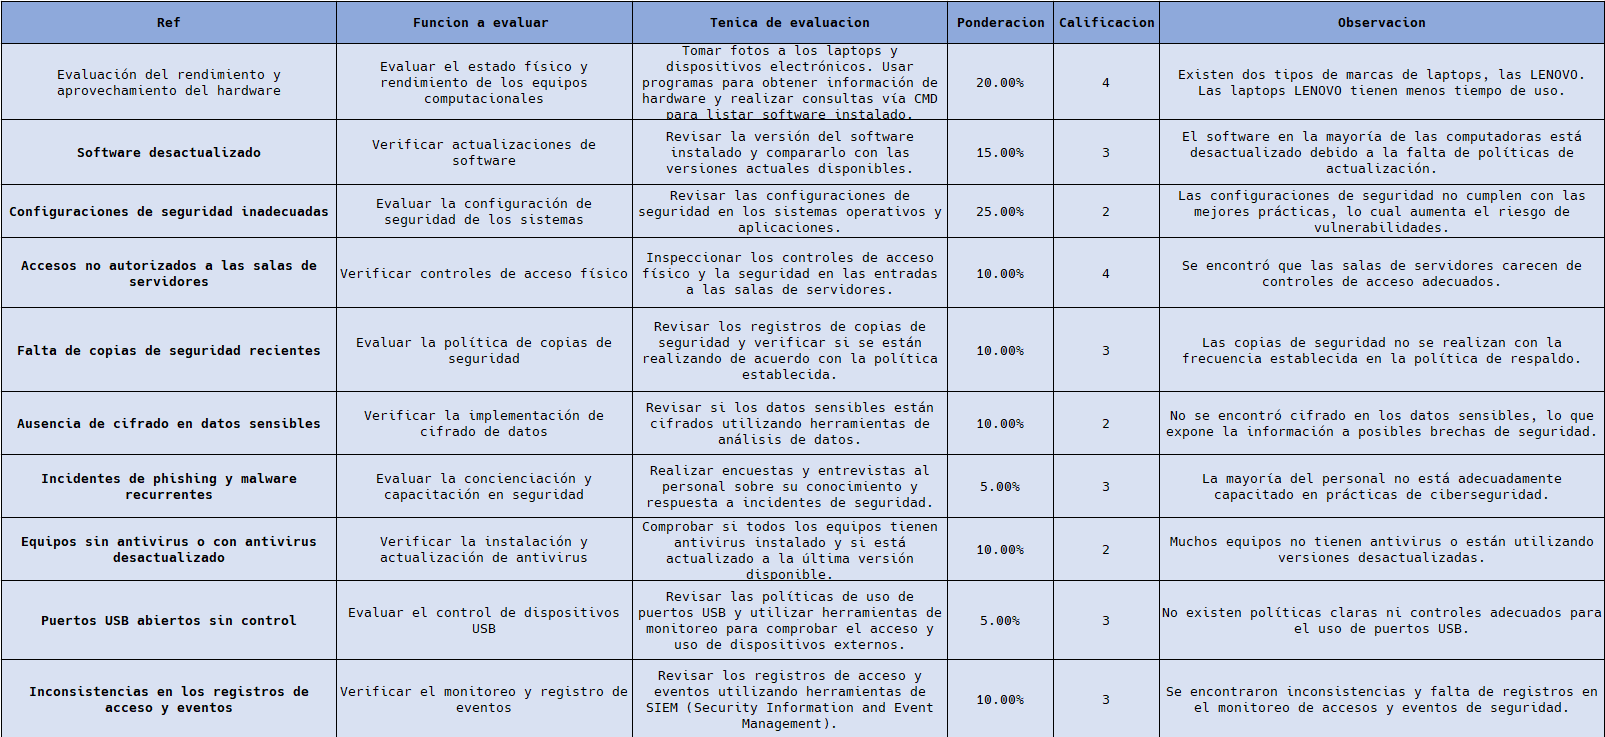
\includegraphics[width=0.8\textwidth]{images/guia.png}
    
\end{figure} 
\FloatBarrier 
%\subsection{Inventario de Software}
%\subsection{Inventario de Hardware}
\subsection{Respaldo de datos}
No tiene respaldo de datos de la información que maneja la organización sin embargo 
Los datos de las base de datos que maneja su pagina web. lo hace una empresa de Tercero

\newpage 



\newpage
\cite{prueba}

\section{Referencias}
\bibliographystyle{apacite}
\bibliography{referencias.bib}


\end{document}